\normalfalse \difficilefalse \tdifficiletrue
\correctionfalse

%\UPSTIidClasse{11} % 11 sup, 12 spé
%\newcommand{\UPSTIidClasse}{12}

\exer{Système de transformation de mouvement  $\star\star$ \label{B2:12:13}}
\setcounter{question}{0}\UPSTIcompetence{B2-12}
\index{Compétence B2-12}
\index{Bielle Manivelle}
\index{Moteur}
\ifcorrection
\else
\marginnote{\textbf{Pas de corrigé pour cet exercice.}}
\fi

\ifprof
\else
Soit le mécanisme suivant. On a $\vect{AB}=R\vect{i_1}$ et $\vect{CA}=H\vect{j_0}$. De plus, 
$R=\SI{30}{mm}$ et $H=\SI{40}{mm}$. 

\begin{center}
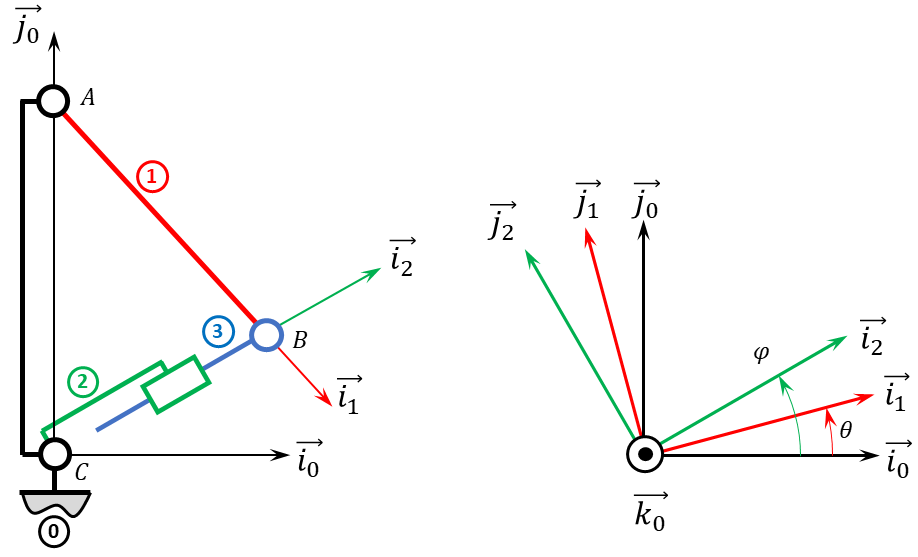
\includegraphics[width=\linewidth]{13_01}
\end{center}
\fi


\question{Tracer le graphe des liaisons.}
\ifprof
\else
\fi

\question{Retracer le schéma cinématique pour $\theta(t)=\dfrac{\pi}{2}\,\text{rad}$.}
\ifprof
\else
\fi

\question{Retracer le schéma cinématique pour $\theta(t)=0\,\text{rad}$.}
\ifprof
\else
\fi

\question{Retracer le schéma cinématique pour $\theta(t)=-\dfrac{\pi}{2}\,\text{rad}$.}
\ifprof
\else
\fi


\question{En déduire la course de la pièce \textbf{3}.}
\ifprof
\else
\fi



\ifprof
\else
\begin{flushright}
\footnotesize{Corrigé  voir \ref{B2:12:13}.}
\end{flushright}%
\fi